\documentclass[a4paper,11pt]{extbook}
\usepackage[a4paper]{geometry}
\geometry{verbose,tmargin=2cm,bmargin=2cm,lmargin=2cm,rmargin=2cm}

\usepackage{fontspec}
%\defaultfontfeatures{Ligatures=TeX}
%\setmainfont{Linux Libertine O}
\setmainfont{FreeSerif}
%\setmonofont{Fira Mono}
\setmonofont{FreeMono}

%\setmainfont{CMU Serif}
%\setmonofont{CMU Typewriter Text}

\setlength{\parindent}{0cm}

\usepackage{float}
\usepackage{graphicx}

\usepackage{hyperref}
\usepackage{url}
\usepackage{xcolor}
\usepackage{amsmath}

\usepackage{minted}
\newminted{julia}{breaklines,fontsize=\footnotesize}
%\newminted{julia}{breaklines}

\definecolor{mintedbg}{rgb}{0.95,0.95,0.95}
\usepackage{mdframed}

\BeforeBeginEnvironment{minted}{\begin{mdframed}[backgroundcolor=mintedbg]}
\AfterEndEnvironment{minted}{\end{mdframed}}

\begin{document}

\title{Electronic Structure Calculation using Plane Wave Basis Set}
\author{Fadjar Fathurrahman}
\date{}
\maketitle

\tableofcontents

\chapter{Introduction}

This document is part of package
{\tt ffr-ElectronicStructure.jl} using plane wave basis set.

{\color{red} WARNING: This document is under heavy construction}

\section{Outline}

First, I will describe the top level description about what
the a typical electronic structure calculation based on density functional
theory is carried out. After that, I will break it apart into
smaller pieces which are hopefully easier to implement and be understood.

In a typical DFT calculation we are trying to solve the so-called Kohn-Sham
equations:
\begin{equation}
H_{KS} \psi_{KS} = e_{KS} \psi_{KS}
\end{equation}

Tasks:
\begin{itemize}
\item Setting up data structure for PW basis set
\item Solving Poisson equation using FFT
\item Solving Schrodinger equation: diagonalization, energy minimization
\item Solving KS equation: SCF and energy minimzation
\end{itemize}



\chapter{Solving Kohn-Sham equations: Version 1}

\begin{enumerate}
\item plane wave basis set
\item solving Poisson equation
\item solving Schrodinger equation
\item solving Kohn-Sham equations
\end{enumerate}

Hamiltonian:
\begin{equation}
H = -\frac{1}{2}\nabla^2 + V_{\mathrm{ps,loc}}(\mathbf{r}) +
V_{\mathrm{Ha}}(\mathbf{r}) + V_{\mathrm{xc}}(\mathbf{r})
\end{equation}



\section{First implementation of plane wave basis: {\tt PWGrid\_01.jl}}

To describe a plane wave basis, we need to define our periodic simulation box
by specifying three lattice vectors. We also need to specify number sampling
points for each lattice vector.
We will store the lattice vector in $3\times3$ matrix.
({\color{red} add convention for lattice vectors, probably using
the same convention as PWSCF input file}).

In file {\tt PWGrid\_01.jl}, we give an implementation of plane wave basis
set, which is encapsulated in a user-defined type {\tt PWGrid}.
An instance of {\tt PWGrid} can be initialize via code like this:

\begin{juliacode}
Ns = [40, 40, 40]  # sampling points
LatVecs = 10*diagm(ones(3))  # lattice vectors for cubic system
pw = PWGrid( Ns, LatVecs )
\end{juliacode}

\subsection{Details of {\tt PWGrid}}

Let's look into details of {\tt PWGrid}.

\verb|PWGrid| is defined like this:

\begin{juliacode}
type PWGrid
  Ns::Array{Int64}
  LatVecs::Array{Float64,2}
  RecVecs::Array{Float64,2}
  Npoints::Int
  Ω::Float64
  r::Array{Float64,2}
  G::Array{Float64,2}
  G2::Array{Float64}
end
\end{juliacode}

Some explanation about these fields follow:

\begin{itemize}

\item {\tt Ns} is an integer array which defines number of sampling points
in each lattice vectors.

\item {\tt LatVecs} is $3\times3$ matrix which defines lattice vectors of
unit cell in real space.

\item {\tt RecVecs} is $3\times3$ matrix which defines lattice vectors of
unit cell in reciprocal space. It is calculated according to \eqref{eq:recvecs}.

\item {\tt Npoints} Total number of sampling points
\item {\tt Ω} Unit cell volume in real space
\item {\tt r} Real space grid points
\item {\tt G} \textbf{G}-vectors
\item {\tt G2} Magnitude of \textbf{G}-vectors

\end{itemize}

The constructor for {\tt PWGrid} is defined as follow.
\begin{juliacode}
function PWGrid( Ns::Array{Int,1}, LatVecs::Array{Float64,2} )
  Npoints = prod(Ns)
  RecVecs = 2*pi*inv(LatVecs')
  Ω = det(LatVecs)
  R,G,G2 = init_grids( Ns, LatVecs, RecVecs )
  return PWGrid( Ns, LatVecs, RecVecs, Npoints, Ω, R, G, G2 )
end
\end{juliacode}

The function {\tt init\_grid()} is defined as follow. It takes
{\tt Ns}, {\tt LatVecs}, and {\tt RecVecs} as the arguments.

\begin{juliacode}
function init_grids( Ns, LatVecs, RecVecs )
\end{juliacode}

First, grid points in real space are initialized:

\begin{juliacode}
  Npoints = prod(Ns)
  r = Array(Float64,3,Npoints)
  ip = 0
  for k in 0:Ns[3]-1
  for j in 0:Ns[2]-1
  for i in 0:Ns[1]-1
    ip = ip + 1
    r[1,ip] = LatVecs[1,1]*i/Ns[1] + LatVecs[2,1]*j/Ns[2]
              + LatVecs[3,1]*k/Ns[3]
    r[2,ip] = LatVecs[1,2]*i/Ns[1] + LatVecs[2,2]*j/Ns[2]
              + LatVecs[3,2]*k/Ns[3]
    r[3,ip] = LatVecs[1,3]*i/Ns[1] + LatVecs[2,3]*j/Ns[2]
              + LatVecs[3,3]*k/Ns[3]
  end
  end
  end
\end{juliacode}

In the next step, grid points in reciprocal space, or \textbf{G}-vectors
and also their squared values are initialized

\begin{juliacode}
  G  = Array(Float64,3,Npoints)
  G2 = Array(Float64,Npoints)
  ip    = 0
  for k in 0:Ns[3]-1
  for j in 0:Ns[2]-1
  for i in 0:Ns[1]-1
    gi = mm_to_nn( i, Ns[1] )
    gj = mm_to_nn( j, Ns[2] )
    gk = mm_to_nn( k, Ns[3] )
    ip = ip + 1
    G[1,ip] = RecVecs[1,1]*gi + RecVecs[2,1]*gj + RecVecs[3,1]*gk
    G[2,ip] = RecVecs[1,2]*gi + RecVecs[2,2]*gj + RecVecs[3,2]*gk
    G[3,ip] = RecVecs[1,3]*gi + RecVecs[2,3]*gj + RecVecs[3,3]*gk
    G2[ip] = G[1,ip]^2 + G[2,ip]^2 + G[3,ip]^2
  end
  end
  end
\end{juliacode}

The function {\tt mm\_to\_nn} defines mapping from real space to Fourier space:

\begin{juliacode}
function mm_to_nn(mm::Int,S::Int)
  if mm > S/2
    return mm - S
  else
    return mm
  end
end
\end{juliacode}

Finally, the variables \verb|r|, \verb|G|, and \verb|G2| are returned.

\begin{juliacode}
  return r,G,G2
\end{juliacode}


\subsection{Visualizing real-space grid points}

In the directory \verb|pwgrid_01|, we visualize grid points in real space
using Xcrysden program. Originally Xcrysden, is meant to visualize crystalline structure,
however, we also can use it to visualize grid points, taking periodic boundary
conditions into consideration.
This is useful to check whether grid points are generated correctly or not.

\begin{figure}
\centering
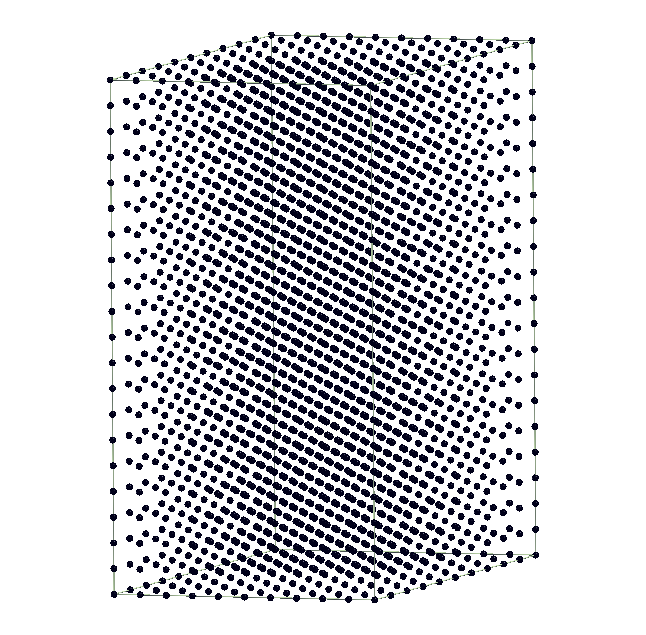
\includegraphics[scale=0.25]{images/R_grid_hexagonal.png}
\par
\end{figure}

\section{Solving Poisson equation}

\begin{mdframed}[backgroundcolor=mintedbg]
\inputminted[breaklines]{julia}{../poisson_01/main.jl}
\end{mdframed}

\section{Calculation of structure factor and Ewald energy: first version}

Structure factor

\begin{juliacode}
# Calculate structure factor
# special case: only for 1 species with Z = 1
function structure_factor( Xpos::Array{Float64,2}, G::Array{Float64,2} )
  Ng = size(G)[2]
  Na = size(Xpos)[2]
  Sf = zeros(Complex128,Ng)
  for ia = 1:Na
    for ig = 1:Ng
      GX = Xpos[1,ia]*G[1,ig] +
           Xpos[2,ia]*G[2,ig] +
           Xpos[3,ia]*G[3,ig]
      Sf[ig] = Sf[ig] + cos(GX) - im*sin(GX)
    end
  end
  return Sf
end
\end{juliacode}

A simple method to calculate Ewald energy

\begin{juliacode}
function calc_ewald( pw::PWGrid, Xpos, Sf; sigma=0.25 )
  #
  const Npoints = pw.Npoints
  const Ω  = pw.Ω
  const r  = pw.r
  const Ns = pw.Ns
  const G2 = pw.G2
  #
  # Generate array of distances
  center = sum(pw.LatVecs,2)/2
  dr = gen_dr( r, center )
  #
  # Generate charge density
  rho = gen_rho( Ns, dr, sigma, Sf )
  intrho = sum(rho)*Ω/Npoints
  #
  # Solve Poisson equation and calculate Hartree energy
  ctmp = 4.0*pi*R_to_G( Ns, rho )
  ctmp[1] = 0.0
  for ip = 2:Npoints
    ctmp[ip] = ctmp[ip] / G2[ip]
  end
  phi = real( G_to_R( Ns, ctmp ) )
  Ehartree = 0.5*dot( phi, rho ) * Ω/Npoints
  #
  Eself = 1.0/(2*sqrt(pi))*(1.0/sigma)*size(Xpos,2)
  return Ehartree - Eself
end
\end{juliacode}

\section{Solving Schrodinger equation}

\subsection{Operators}

Kinetic energy operators (multicolumns):

\begin{juliacode}
function op_K( pw::PWGrid, psi::Array{Complex128,2} )
  out = zeros(Complex128,size(psi))
  Ncol = size(psi,2)
  Ω = pw.Ω
  G2 = pw.G2
  Npoints = pw.Npoints
  for is = 1:Ncol
    for ip = 1:Npoints
      out[ip,is] = psi[ip,is]*G2[ip]
    end
  end
  return 0.5*out
end
\end{juliacode}

Applying potential

\begin{juliacode}
function op_Vpot( pw::PWGrid, Vpot, psi::Array{Complex128,2} )
  Ns = pw.Ns
  Ω = pw.Ω
  Npoints = prod(Ns)
  # get values of psi in real space grid via forward transform
  ctmp = G_to_R( Ns, psi )
  return R_to_G( Ns, Diagprod(Vpot, ctmp) )
end
\end{juliacode}

Function {\tt Diagprod}:

\begin{juliacode}
function Diagprod( a,B )
  Ncol    = size(B)[2]
  Npoints = size(B)[1]
  out = zeros( Complex128, size(B) )
  for ic = 1:Ncol
    for ip = 1:Npoints
      out[ip,ic] = a[ip]*B[ip,ic]
    end
  end
  return out
end
\end{juliacode}

Hamiltonian operator:

\begin{juliacode}
function op_H( pw, Vpot, psi )
  return op_K( pw, psi ) + op_Vpot( pw, Vpot, psi )
end
\end{juliacode}


\subsection{Gradient calculation}

Gradient of energy with respect to wave function

Not using occupation number

\begin{juliacode}
function calc_grad( pw::PWGrid, Vpot, psi::Array{Complex128,2} )
  Npoints = size(psi)[1]
  Nstates = size(psi)[2]
  Ω = pw.Ω
  Ns = pw.Ns
  #
  grad = zeros( Complex128, Npoints, Nstates )
  H_psi = op_H( pw, Vpot, psi )
  for i = 1:Nstates
    grad[:,i] = H_psi[:,i]
    for j = 1:Nstates
      grad[:,i] = grad[:,i] - dot( psi[:,j], H_psi[:,i] ) * psi[:,j]
    end
  end
  return grad
end
\end{juliacode}



\subsection{Calculation of charge density}

\begin{juliacode}
function calc_rho( pw::PWGrid, psi::Array{Complex128,2} )
  Ω = pw.Ω
  Ns = pw.Ns
  Npoints = pw.Npoints
  Nstates = size(psi)[2]
  #
  ρ = zeros(Complex128,Npoints)
  # Transform to real space
  psiR = G_to_R(Ns,psi)
  # orthonormalization in real space
  ortho_gram_schmidt!(Nstates,psiR); scale!(sqrt(Npoints/Ω),psiR)
  for is = 1:Nstates
    for ip = 1:Npoints
      ρ[ip] = ρ[ip] + conj(psiR[ip,is])*psiR[ip,is]
    end
  end
  return real(ρ)
end
\end{juliacode}


\subsection{Calculation of total energy}


\begin{juliacode}
function calc_Etot( pw::PWGrid, Vpot, psi::Array{Complex128,2} )
  Ω = pw.Ω
  Npoints = pw.Npoints
  Nstates = size(psi)[2]
  Kpsi = op_K( pw, psi )
  Ekin = 0.0
  for is = 1:Nstates
    Ekin = Ekin + real( dot( psi[:,is], Kpsi[:,is] ) )
  end
  # Calculate in real space
  rho = calc_rho( pw, psi )
  Epot = dot( rho, Vpot ) * Ω/Npoints
  Etot = Ekin + Epot
  return Etot
end
\end{juliacode}


\subsection{Energy minimization with steepest descent}

\begin{juliacode}
function Sch_solve_Emin_sd( pw::PWGrid, Vpot, psi::Array{Complex128,2};
                            NiterMax=1000 )
  α = 3e-5
  Etot_old = 0.0
  Etot = 0.0
  for iter = 1:NiterMax
    psi = psi - α*calc_grad( pw, Vpot, psi )
    psi  = ortho_gram_schmidt(psi)
    Etot = calc_Etot( pw, Vpot, psi )
    conv = abs(Etot-Etot_old)
    if conv < 1e-6
      break
    end
    Etot_old = Etot
  end
  return psi, Etot
end
\end{juliacode}


\subsection{Energy minimization with conjugate gradient}

\begin{juliacode}
function Sch_solve_Emin_cg( pw::PWGrid, Vpot, psi::Array{Complex128,2};
                            NiterMax=1000 )
  #
  Npoints = size(psi)[1]
  Nstates = size(psi)[2]
  d = zeros(Complex128, Npoints, Nstates)
  g_old  = zeros(Complex128, Npoints, Nstates)
  d_old  = zeros(Complex128, Npoints, Nstates)
  Kg     = zeros(Complex128, Npoints, Nstates)
  Kg_old = zeros(Complex128, Npoints, Nstates)
  #
  α_t = 1.e-5
  β = 0.0
  Etot_old = 0.0
  Etot = 0.0
  #
  for iter = 1:NiterMax
    g = calc_grad( pw, Vpot,  psi)
    nrm = 0.0
    for is = 1:Nstates
      nrm = nrm + real( dot( g[:,is], g[:,is] ) )
    end
    Kg = Kprec(pw,g)
    if iter != 1
      β = real( sum( conj(g) .* Kg ) ) / real( sum( conj(g_old) .* Kg_old ) )
    end
    d = -Kg + β * d_old
    psic = ortho_gram_schmidt(psi + α_t*d)
    gt = calc_grad( pw, Vpot, psic )
    denum = real(sum(conj(g-gt).*d))
    if denum != 0.0
      α = abs(α_t*real(sum(conj(g).*d))/denum)
    else
      α = 0.0
    end
    # Update wavefunction
    psi = psi[:,:] + α*d[:,:]
    psi = ortho_gram_schmidt(psi)
    Etot = calc_Etot( pw, Vpot, psi )
    diff = abs(Etot-Etot_old)
    @printf("E step %8d = %18.10f %18.10f %18.10f\n", iter, Etot, diff, nrm/Nstates)
    if diff < 1e-6
      @printf("CONVERGENCE ACHIEVED\n")
      break
    end
    g_old = copy(g)
    d_old = copy(d)
    Kg_old = copy(Kg)
    Etot_old = Etot
  end
  return psi, Etot
end
\end{juliacode}


{\color{red}
Using energy minimization:

Introduction to minimization

simple 2D minimization, using steepest-descent and conjugate gradient
method

Using iterative diagonalization: Davidson and LOBPCG

background information about iterative diagonalization

Eigenvalue problems

}





\chapter{Solving Kohn-Sham equations: Version 2}

Improvements

Hamiltonian is still the same as the Version 1.
\begin{equation}
H = -\frac{1}{2}\nabla^2 + V_{\mathrm{ps,loc}}(\mathbf{r}) +
V_{\mathrm{Ha}}(\mathbf{r}) + V_{\mathrm{xc}}(\mathbf{r})
\end{equation}


\begin{juliacode}
  const PWGRID_VERSION = 2

  type GVectorsW
    Ngwx::Int
    idx_gw2r::Array{Int}
  end

  type GVectors
    Ng::Int
    G::Array{Float64,2}
    G2::Array{Float64}
  end

  type PWGrid
    Ns::Array{Int64}
    LatVecs::Array{Float64,2}
    RecVecs::Array{Float64,2}
    Ω::Float64
    r::Array{Float64,2}
    gvec::GVectors
    gvecw::GVectorsW
  end

  function PWGrid( Ns, LatVecs::Array{Float64,2} )

    if any( Ns%2 .== 1 )
      @printf("Error: Ns must be even numbers\n")
      exit()
    end

    RecVecs = 2*pi*inv(LatVecs')
    Ω = det(LatVecs)
    #
    LatVecsLen = zeros(3)
    LatVecsLen[1] = norm(LatVecs[1,:])
    LatVecsLen[2] = norm(LatVecs[2,:])
    LatVecsLen[3] = norm(LatVecs[3,:])

    Npoints = prod(Ns)
    r = init_grid_R( Ns, LatVecs )

    gvec = init_grid_G( Ns, RecVecs )
    gvecw = init_gvecw( Ns, gvec.G2 )

    return PWGrid( Ns, LatVecs, RecVecs, Ω, r, gvec, gvecw )
  end

  function mm_to_nn(mm::Int,S::Int)
    if mm > S/2
      return mm - S
    else
      return mm
    end
  end


  function init_grid_G( Ns, RecVecs )

    Ng = prod(Ns)

    G  = Array(Float64,3,Ng)
    G2 = Array(Float64,Ng)

    ig = 0
    for k in 0:Ns[3]-1
    for j in 0:Ns[2]-1
    for i in 0:Ns[1]-1
      ig = ig + 1
      gi = mm_to_nn( i, Ns[1] )
      gj = mm_to_nn( j, Ns[2] )
      gk = mm_to_nn( k, Ns[3] )
      G[1,ig] = RecVecs[1,1]*gi + RecVecs[2,1]*gj + RecVecs[3,1]*gk
      G[2,ig] = RecVecs[1,2]*gi + RecVecs[2,2]*gj + RecVecs[3,2]*gk
      G[3,ig] = RecVecs[1,3]*gi + RecVecs[2,3]*gj + RecVecs[3,3]*gk
      G2[ig] = G[1,ig]^2 + G[2,ig]^2 + G[3,ig]^2
    end
    end
    end

    return GVectors( Ng, G, G2 )
  end

  function init_gvecw( Ns, G2 )
    edges = find_edges( Ns )
    G2mx = minimum( G2[edges] )
    #@printf("G2mx = %f\n", G2mx)
    @printf("ecutwfc_Ry = %f\n", G2mx/4)
    idx_gw2r = findn( G2 .< G2mx/4 )
    Ngwx = length(idx_gw2r)
    return GVectorsW( Ngwx, idx_gw2r )
  end

  function find_edges( Ns )
    eS = Ns/2 + 0.5
    edges = []
    ip = 1
    for k in 0:Ns[3]-1
    for j in 0:Ns[2]-1
    for i in 0:Ns[1]-1
      ei = abs(i - eS[1])
      ej = abs(j - eS[2])
      ek = abs(k - eS[3])
      # if any of i, j, or k is equal to Ns/2 or Ns/2+1
      if ei < 1.0 || ej < 1.0 || ek < 1.0
        push!(edges,ip)
      end
      ip = ip + 1
    end
    end
    end
    return edges
  end


  function init_grid_R( Ns, LatVecs )
    #
    Npoints = prod(Ns)
    #
    R = Array(Float64,3,Npoints)
    ip = 0
    for k in 0:Ns[3]-1
    for j in 0:Ns[2]-1
    for i in 0:Ns[1]-1
      ip = ip + 1
      R[1,ip] = LatVecs[1,1]*i/Ns[1] + LatVecs[2,1]*j/Ns[2] + LatVecs[3,1]*k/Ns[3]
      R[2,ip] = LatVecs[1,2]*i/Ns[1] + LatVecs[2,2]*j/Ns[2] + LatVecs[3,2]*k/Ns[3]
      R[3,ip] = LatVecs[1,3]*i/Ns[1] + LatVecs[2,3]*j/Ns[2] + LatVecs[3,3]*k/Ns[3]
    end
    end
    end
    #
    return R
  end
\end{juliacode}

A slight modification for {\tt Poisson_solve}

\begin{juliacode}
function Poisson_solve( PW::PWGrid, rhoR )
  G2 = PW.gvec.G2
  Ns = PW.Ns
  Npoints = prod(Ns)
  ctmp = 4.0*pi*R_to_G( Ns, rhoR )
  ctmp[1] = 0.0
  for ip = 2:Npoints
    ctmp[ip] = ctmp[ip]/G2[ip]
  end
  return ctmp
end
\end{juliacode}

Version 2

\begin{juliacode}
function calc_ewald( pw::PWGrid, Sf, Xpos, Nspecies::Int, atm2species,
                     Zv::Array{Float64}; sigma=nothing )
  #
  Ω  = pw.Ω
  r  = pw.r
  Ns = pw.Ns
  G2 = pw.gvec.G2
  Npoints = prod(Ns)
  LatVecs = pw.LatVecs
  #
  # Generate array of distances
  dr = gen_dr_center( r, LatVecs )
  #
  # Generate charge density
  #
  if sigma==nothing
    sigma = 0.25*ones(Nspecies)
  end
  #
  g1  = zeros( Float64, Npoints )
  rho_is = zeros( Float64, Npoints, Nspecies )
  Rho = zeros(Float64, Npoints)
  #
  for isp = 1:Nspecies
    c1 = 2*sigma[isp]^2
    cc1 = sqrt(2*pi*sigma[isp]^2)^3
    for ip=1:Npoints
      g1[ip] = exp(-dr[ip]^2/c1)/cc1
    end
    #
    g1 = Zv[isp] * g1[:]
    #
    ctmp = R_to_G( Ns, g1 )
    for ip = 1:Npoints
      ctmp[ip] = ctmp[ip]*Sf[ip,isp]
    end
    rho_is[:,isp] = real( G_to_R(Ns, ctmp) )
    intrho = sum(rho_is[:,isp])*Ω/Npoints
    Rho[:] = Rho[:] + rho_is[:,isp]
  end

  intrho = sum(Rho)*Ω/Npoints
  #
  # Solve Poisson equation and calculate Hartree energy
  ctmp = 4.0*pi*R_to_G( Ns, Rho )
  ctmp[1] = 0.0
  for ip = 2:Npoints
    ctmp[ip] = ctmp[ip] / G2[ip]
  end
  phi = real( G_to_R( Ns, ctmp ) )
  Ehartree = 0.5*dot( phi, Rho ) * Ω/Npoints
  #
  Eself = 0.0
  Natoms = size(Xpos)[2]
  for ia = 1:Natoms
    isp = atm2species[ia]
    Eself = Eself + Zv[isp]^2/(2*sqrt(pi))*(1.0/sigma[isp])
  end
  E_nn = Ehartree - Eself
  return E_nn
end
\end{juliacode}



\chapter{Formulae}

Plane wave basis $b_{\alpha}(\mathbf{r})$:
\begin{equation}
b_{\alpha}(\mathbf{r}) = \frac{1}{\sqrt{\Omega}} e^{\mathbf{G}_{\alpha}\cdot\mathbf{r}}
\end{equation}

Lattice vectors of unit cell in reciprocal space:
\begin{equation}\label{eq:recvecs}
\mathbf{b} = 2\pi\left( a^{T} \right)^{-1}
\end{equation}

\textbf{G}-vectors:
\begin{equation}
\mathbf{G} = i \mathbf{b}_{1} + j \mathbf{b}_{2} + k \mathbf{b}_{3}
\end{equation}

Structure factor:
\begin{equation}
S_{I}(\mathbf{G}) = \sum_{\mathbf{G}} e^{ -\mathbf{G}\cdot\mathbf{X}_{I} }
\end{equation}



\end{document}
